% SECTION 18: Lattice Calculations of the Hadron Spectrum
% R. Gupta, "Introduction to Lattice QCD" (arXiv:hep-lat/9807028)

\chapter{Lattice Calculations of the Hadron Spectrum}

Successful calculations of the spectrum will test QCD. The basic steps in the lattice analysis are discussed in Sections~4 and~17. For a given set of input parameters, the mass of a given state is determined from the rate of exponential fall-off of the connected 2-point correlation function
\begin{equation}
\Gamma(\tau) \equiv \langle O_f(\tau) O_i(0) \rangle - \langle O_f \rangle \langle O_i \rangle
= \sum_n \frac{\langle 0 | O_f | n \rangle \langle n | O_i | 0 \rangle}{2 M_n}\, e^{-M_n \tau}.
\label{eq:2pt}
\end{equation}

We shall assume that the sum over $n$ is restricted to the desired state by (i) optimizing $O_i$ and $O_f$ to get a large overlap with the wave function, i.e.\ make desired state $\langle n | O | 0 \rangle$ large and the rest small, (ii) increasing the statistics so that the signal extends to large enough $\tau$ at which any remaining contamination from higher states is negligible; and (3) making a zero-momentum projection on either $O_i$ or $O_f$. I shall further assume that the spectrum of possible states is discrete and has a mass-gap. Then, in order to extract $M$ it is useful to define an effective mass
\begin{equation}
M_{eff}(\tau) = \log\!\left( \frac{\Gamma(\tau-1)}{\Gamma(\tau)} \right)
\label{eq:meff}
\end{equation}
which, in the limit $\tau \to \infty$, converges to the desired value. The anatomy of the behavior of $M_{eff}(\tau)$ for two different states (pion and nucleon) and for two different choices of $O_i$ and $O_f$ are shown in Figs.~\ref{fig:22} and~\ref{fig:23}. The points to note are:
\begin{itemize}
\item The convergence to the asymptotic value $M$ can be from above or below depending on the choice of $O$. Only for $O_f = O_i^\dagger$ is the correlation function positive definite and the convergence is monotonic and from above.
\item For $O_f \neq O_i^\dagger$, the convergence depends on subtle cancellations between contributions of various states. The relative signs are given by the product of the two amplitudes $\langle n | O_f | 0 \rangle \langle n | O_i | 0 \rangle$. Since this sign for state $|n\rangle$ can be plus or minus, the convergence is neither guaranteed to be monotonic nor from above.
\end{itemize}

\begin{figure}[htbp]
\centering
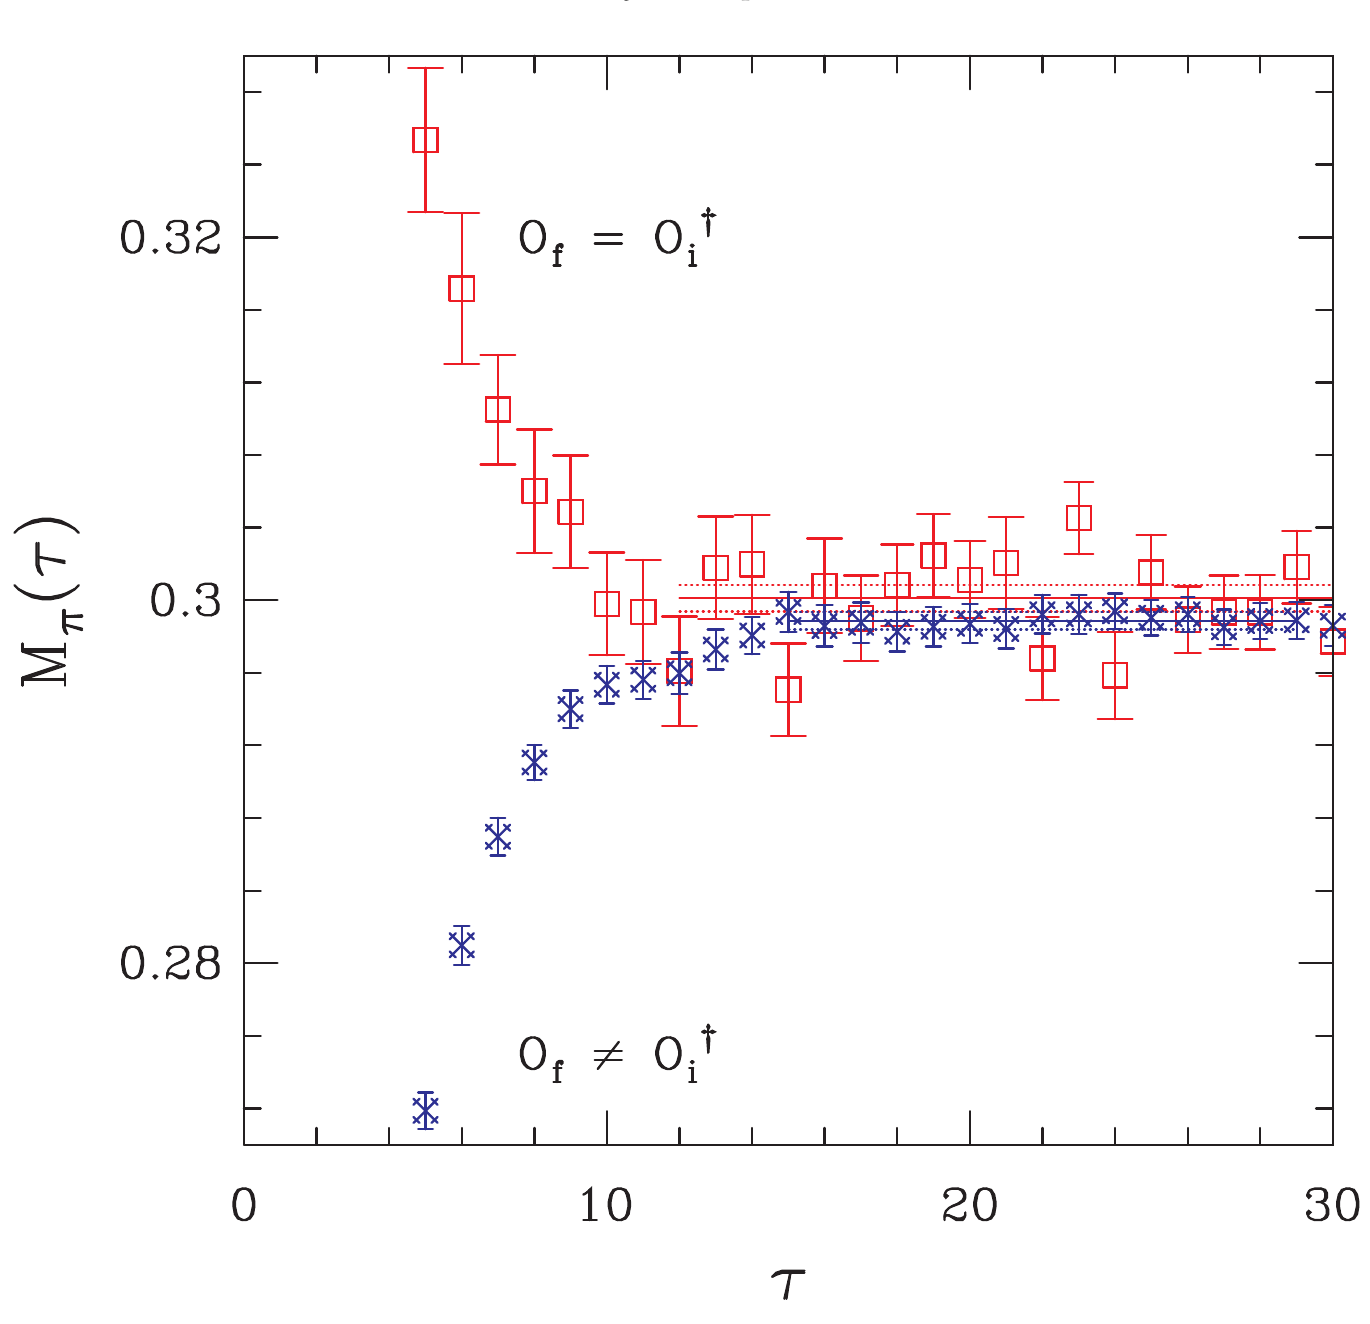
\includegraphics[width=0.8\textwidth]{images/fig22.png}
\caption{Effective mass plots for $M_\pi$ versus $\tau$. The horizontal lines denote the estimate of the asymptotic value of $M$ and the range of the plateau used in the fits, while the dotted lines show the error. The squares denote data for smeared-smeared interpolating operators ($O_f = O_i^\dagger$), while fancy crosses show data with wall-local operators.}
\label{fig:22}
\end{figure}

\begin{itemize}
\item The contribution of excited states is most obvious at small $\tau$, where $M_{eff}$ varies rapidly before flattening out. For $\tau$ in this flat (called plateau) region one assumes that, within the numerical precision, only the lowest state contribution is significant.
\item The location in $\tau$ of the onset and the length of the plateau region depends on the interpolating operators.
\item For a finite statistical sample the plateau region is not flat but the data usually exhibit correlated fluctuations [158]. Therefore, unless the plateau is long enough that the fit can average over a few cycles, the extracted $M_{eff}$ can be biased by these statistical fluctuations.
\end{itemize}

\begin{figure}[htbp]
\centering
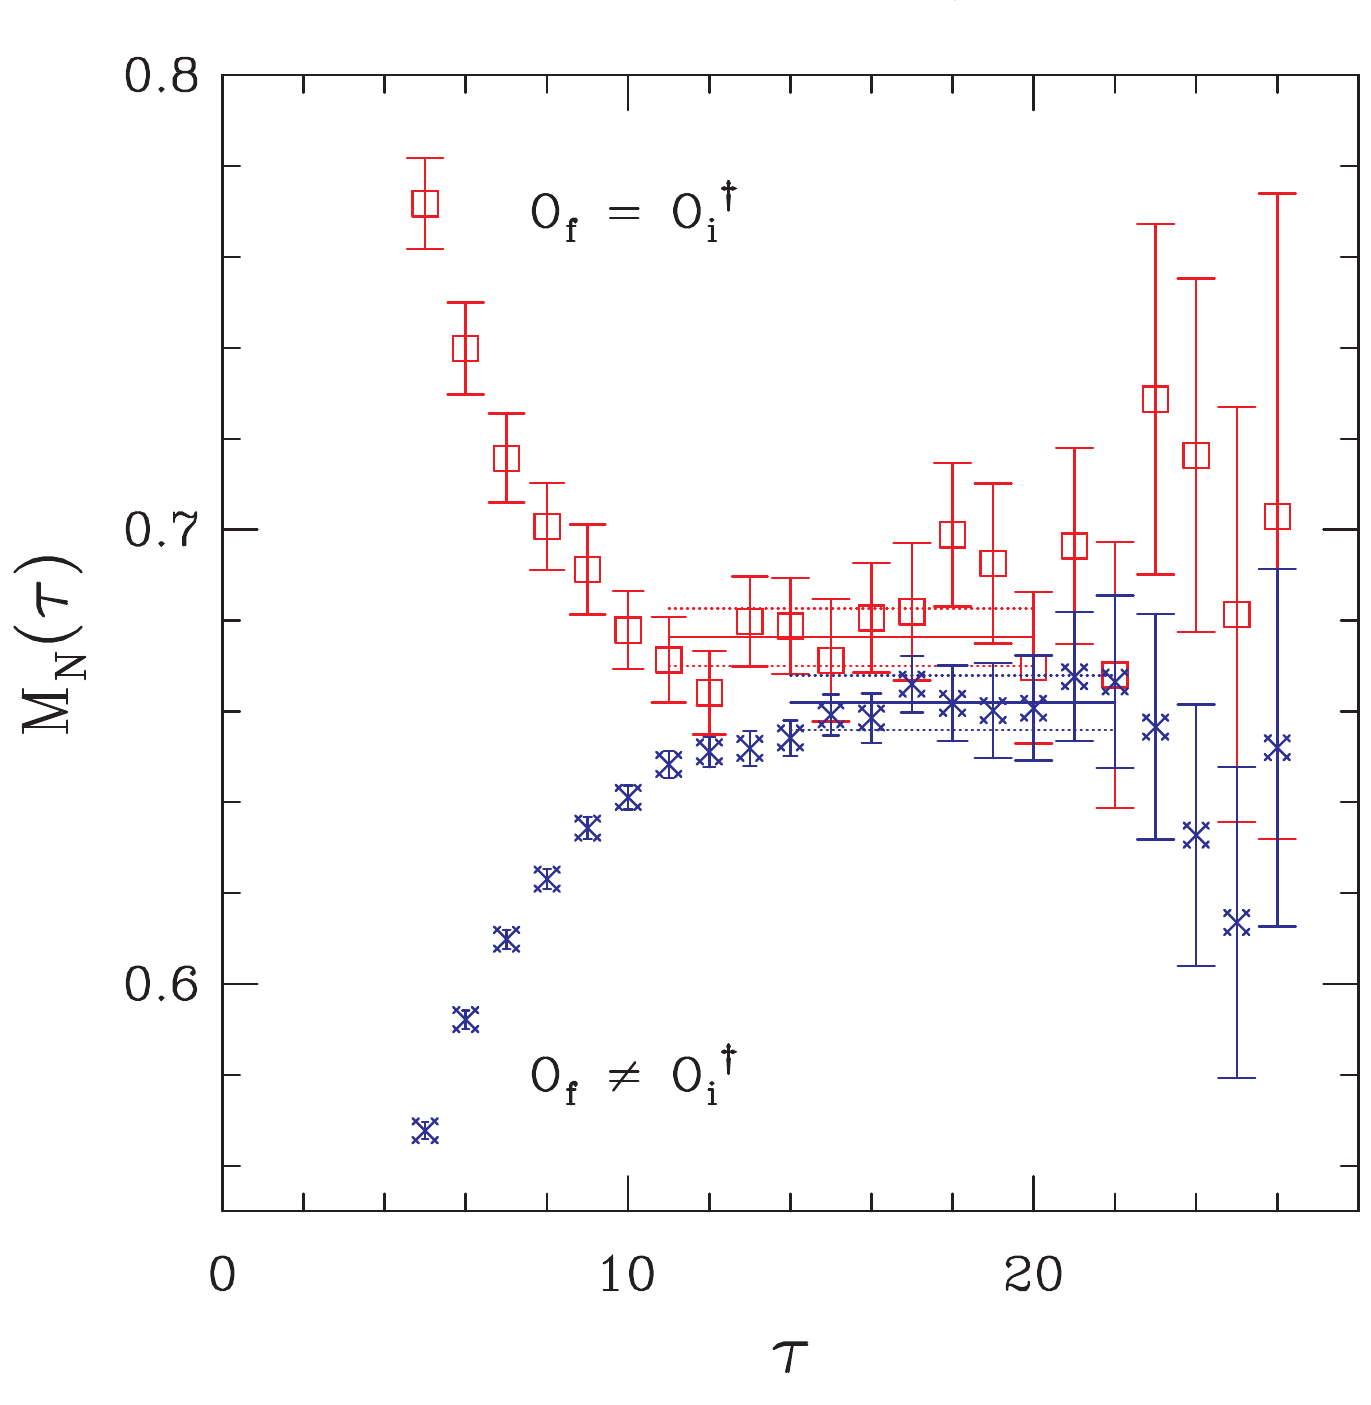
\includegraphics[width=0.8\textwidth]{images/fig23.png}
\caption{Effective mass plots for $M_N$ versus $\tau$. The rest is the same as in Fig.~\ref{fig:22}.}
\label{fig:23}
\end{figure}

\begin{itemize}
\item The statistical errors grow with $\tau$, except for the case of the pion. The reason for this was elucidated by Lepage in [159] and a synopsis of his argument is as follows. For a state with $N$ valence quark lines, where $N = 2(3)$ for mesons (baryons), the errors are controlled by the square of the correlator which has $2N$ lines. The state of lowest energy in the squared correlator is, therefore, two pions for mesons and three pions for baryons. Thus, while the signal decreases as $\exp(-M \tau)$, the noise only decreases as $\exp(-M_\pi \tau \times N/2)$. Consequently, all states for which $M > N M_\pi / 2$ the errors will increase with $\tau$. The only exception to this condition is the pion for which the signal and noise have the same $\tau$ dependence.
\item In cases where there is no clear plateau (the signal does not extend far enough in $\tau$), one can make a fit to a larger range of $\tau$ by including the contribution of higher (radial) states in the sum in Eq.~\eqref{eq:2pt}. This is illustrated in Fig.~\ref{fig:24} for a two state fit which involves four free parameters, two amplitudes and two masses. The amplitude and mass of the excited state are less well constrained as they are trying to mimic the effect of a number of states, consequently such fits may show significant dependence on the range of $\tau$ selected. One can refine the excited state parameters by iteratively improving single state fits to $\Gamma(\tau) - \Gamma_0(\tau)$ at short $\tau$ and to the ground state $\Gamma_0(\tau)$ at large $\tau$ until the whole range is covered. A better approach to gain confidence in ground state parameters is to make simultaneous fits to a matrix of correlation functions created with different source and sink operators with the same quantum numbers. For a matrix with $m$ ($n$) distinct sources (sinks) the simultaneous fit is more constraining as it involves $m + n$ amplitudes but a single common mass.
\end{itemize}

\begin{figure}[htbp]
\centering
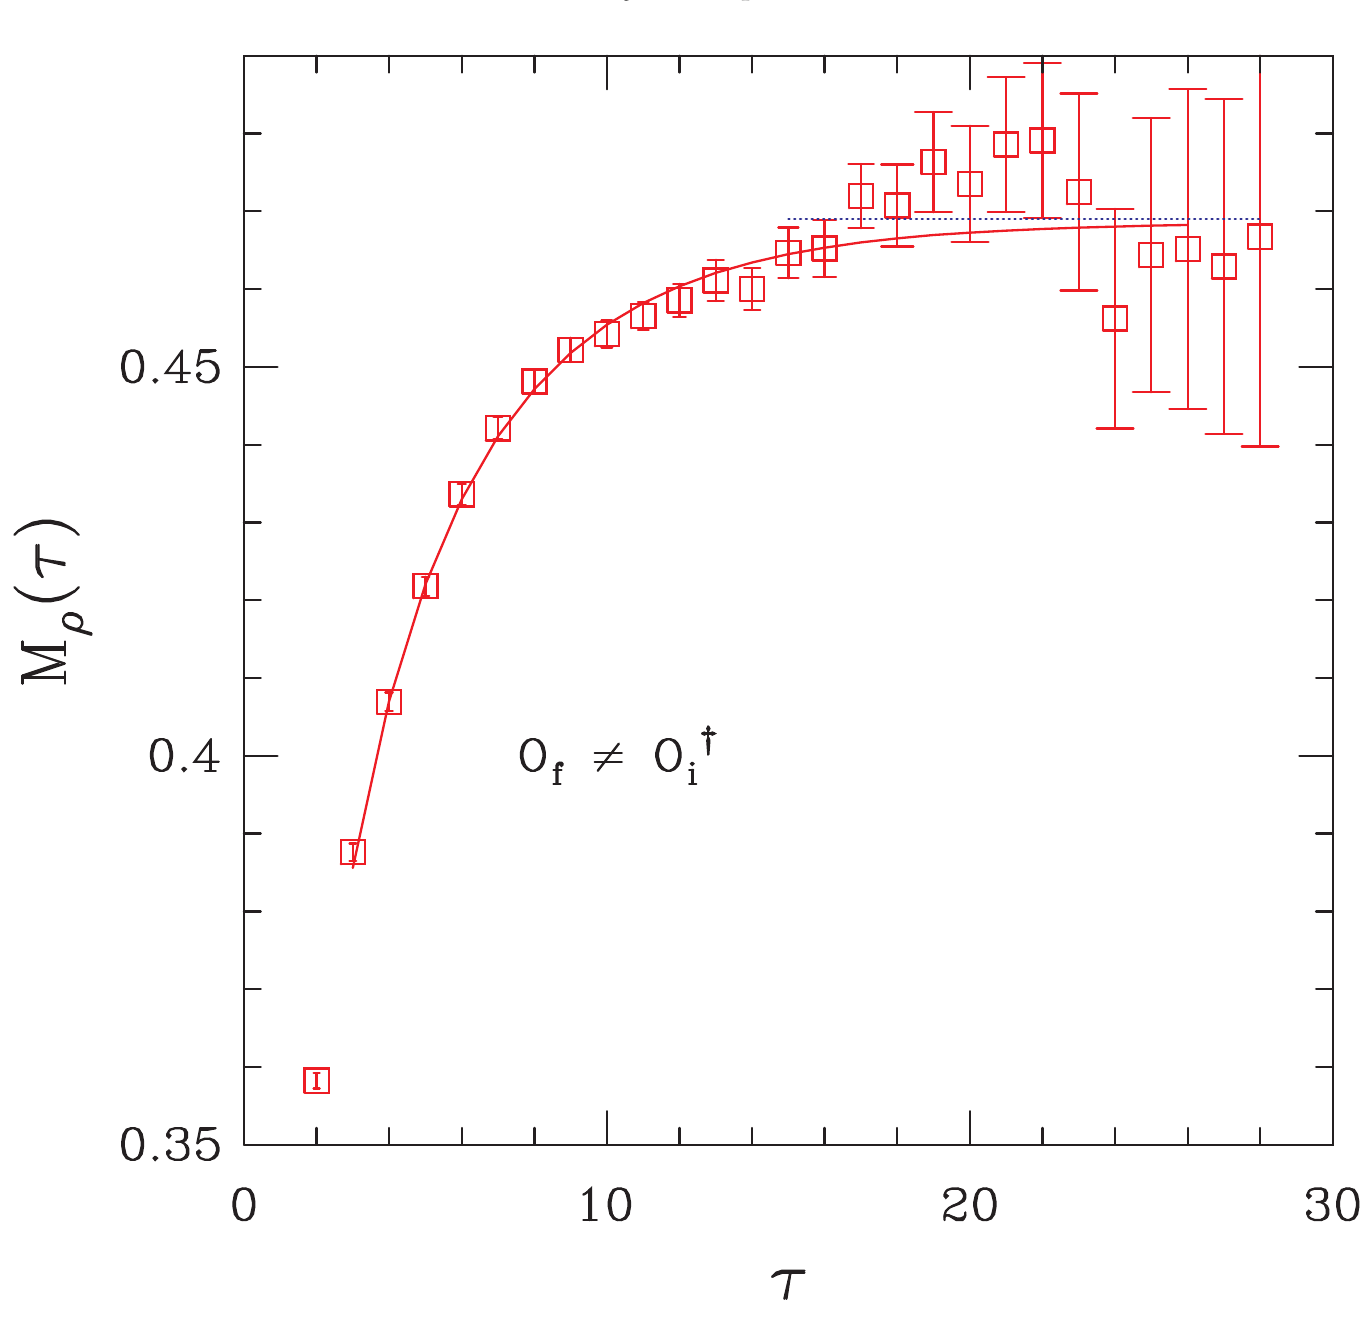
\includegraphics[width=0.8\textwidth]{images/fig24.png}
\caption{Effective mass plots for $M_\rho$ versus $\tau$ for the wall-local source. Since there is no clear plateau, a fit including two states is made to $3 \leq \tau \leq 26$. From such fits the masses of $\rho$ and $\rho^*$ are obtained. The mass of the $\rho$ from the 2-state fit is consistent with that from a single state fit to data at $\tau > 15$ (blue dotted line).}
\label{fig:24}
\end{figure}

To summarize, we mostly extract $M$ from fits to an intermediate range of $\tau$, the ``plateau'' region, where $M_{eff}$ is essentially independent of $\tau$. At small $\tau$ the influence of excited states is large, while at large $\tau$ the statistical noise overwhelms the signal. Accuracy of the result depends on the presence of a plateau extending over a large range of $\tau$ that averages a few cycles of correlated fluctuations. The data in Figs.~\ref{fig:22}, \ref{fig:23}, and \ref{fig:24} show that, with 170 lattices of size $32^3 \times 64$ at $1/a = 2.3$ GeV, this is true for the pion but marginal for other states like the vector mesons and baryons. Our present estimate is that roughly 1000 independent lattices are necessary to get a reliable signal that leads to 0.1--0.4\% accuracy in baryon masses with quark masses in the range $m_s - m_s/4$ respectively.

Assuming that the above steps have been carried out and we have reliable estimates for hadron masses as a function of quark masses, $a$, $L$, and the number $n_f$ of dynamical flavors, we are finally in a position to compare them to experimental data.

\section{Status of the Light Meson and Baryon Spectrum}

The first test of QCD is to reproduce the masses of pseudoscalar mesons (PS = $\{\pi, K, \eta\}$), vector mesons (V = $\{\rho, K^*, \omega, \phi\}$), octet baryons ($B_8 = \{N, \Sigma, \Xi, \Lambda\}$), and decuplet baryons ($B_{10} = \{\Delta, \Sigma^*, \Xi^*, \Omega\}$) from simulations with four input parameters $m_u$, $m_d$, $m_s$, and $\alpha_s$. I will assume that the lattices are large enough that finite size effects can be neglected. The remaining important issues are
\begin{itemize}
\item Simulations have mainly been done in the quenched approximation. Rather than testing QCD, these calculations quantify the accuracy of QQCD.
\item Isospin breaking effects and electromagnetic contributions are neglected.
\item Simulations have been done with unphysical values of quark masses, typically in the range $[2m_s - m_s/4]$. To get physical results the data are extrapolated to $m = (m_u + m_d)/2$ using functional forms predicted by (quenched) chiral perturbation theory.
\end{itemize}

The first step in the analyses is to extrapolate the data to physical values of $m$ and $m_s$. The simplest Ans\"atze are the lowest order chiral expressions
\begin{equation}
\begin{aligned}
M_{PS}^2 a^2 &= B_{PS} a^2 (m_1 + m_2)/2 + \cdots, \\
M_V a &= A_V + B_V a (m_1 + m_2)/2 + \cdots, \\
M_\Sigma a &= A_N + 4F m a + 2(F - D) m_s a + \cdots, \\
M_\Lambda a &= A_N + 4(F - D/3) m a + 2(F + D/3) m_s a + \cdots, \\
M_{10} a &= A_{10} + B_{10} a (m_1 + m_2 + m_3)/3 + \cdots.
\end{aligned}
\label{eq:chiral}
\end{equation}

From these fits we determine the constants $A_V$, $A_N$, $A_{10}$ and $B_{PS}$, $B_V$, $F$, $D$, $B_{10}$. Then using a suitable set, for example $A_V$, $B_{PS}$, $B_V$ or $A_{10}$, $B_{PS}$, $B_{10}$, we fix the three input parameters $1/a$, $m$, $m_s$. Unless otherwise stated the following discussion will assume that $m$, $a$, and $m_s$ have been fixed using $M_\pi$, $M_\rho$, and $M_\phi$ (or equivalently $M_{K^*}$) respectively. The question then is --- how well do the masses of the remaining states compare with experimental numbers?

This simple analysis to test QCD (or to quantify the quenched approximation) can fall short in two ways. First, the data could show significant deviations from the linear relations Eq.~\eqref{eq:chiral}. In that case the analysis becomes much more elaborate due to the increase in the number of free parameters; the possible leading non-linear terms include $O(m^2)$ corrections and chiral logarithms. To disentangle these requires very precise data at a number of values of $m_q$ in the range $m_s/4 - 3m_s$, however, such a possibility of physics richer than that predicted by the ``naive'' quark model is exciting. The second possible failing is that different sets of states used to fix $a$, $m$, $m_s$ give different results. There could be three reasons for this failure: (i) The coefficients extracted from simulations at the significantly heavier values of $m_q$ change as the quark masses are decreased; (ii) the differences are artifacts of discretization errors and vanish in the limit $a = 0$; (3) quenching errors. The current data show evidence for non-linearities in fits in $m_q$ [156,160]. Also, the $a$, $m$, $m_s$ extracted from different sets are significantly different, and all three causes listed above contribute. As a result the focus of current analyses has been to first disentangle and quantify the contributions of the various artifacts. I will briefly illustrate these effects.

Let me start with evidence for non-linear terms in the chiral fits. Fig.~\ref{fig:25} is an example of the behavior of the vector meson mass as a function of the quark mass [156]. The plot makes it clear that in order to quantify the deviations one needs very precise data over a large range of $m_q$. With a statistical accuracy of $\sim 0.5\%$, a linear fit works for $0.02 \leq ma \leq 0.04$ corresponding to $50 \leq m \leq 100$ MeV, but not for the full range. The leading chiral corrections are proportional to $m^{3/2}$ from chiral loops, and $m^2$. Including either term allows fits over the full range, and the data are not precise enough to distinguish between them. The effect of these non-linearities seems to be small, for example the change in $M_\rho$, after extrapolation to $m$, is $\sim < 1\%$ on including either of the higher order terms in the fit.

\begin{figure}[htbp]
\centering
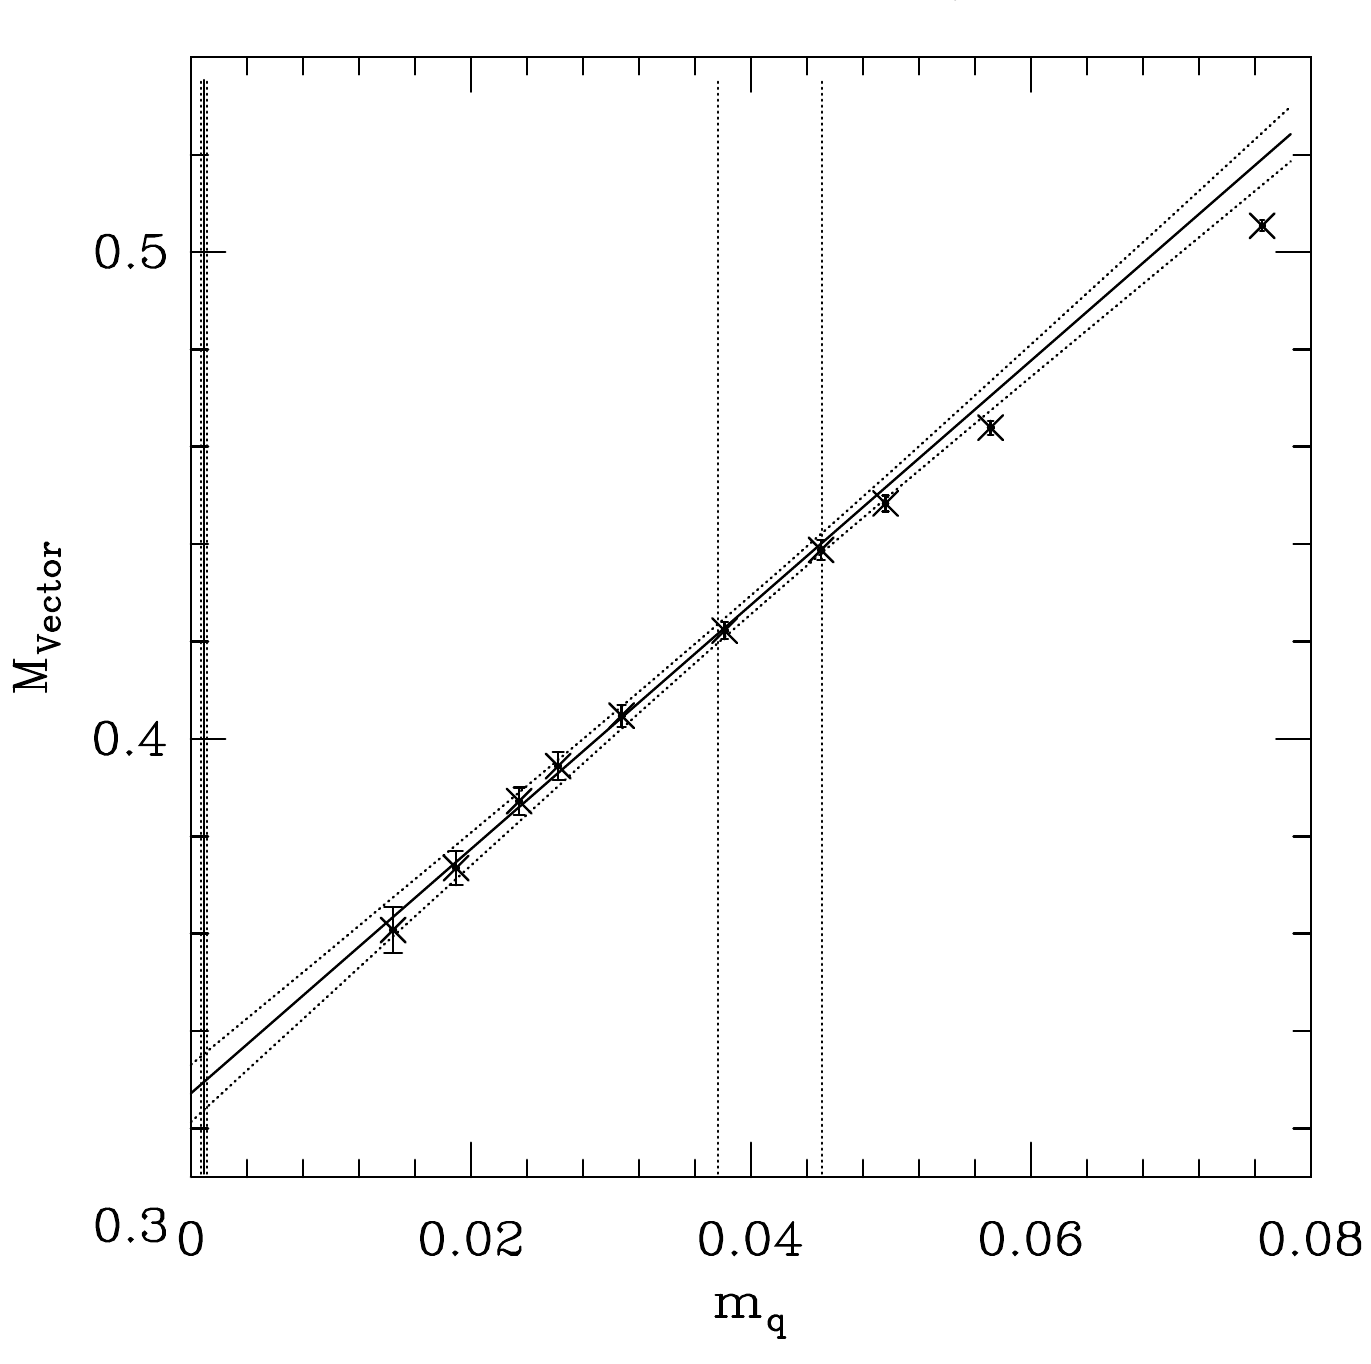
\includegraphics[width=0.8\textwidth]{images/fig25.png}
\caption{Plot of $M_{vector}$ versus the quark mass $m$. The data, reproduced from [156], were obtained on $32^3 \times 64$ quenched lattices at $\beta \equiv 6/g^2 = 6$ corresponding to $1/a = 2.33(4)$ GeV. The linear fit is to the lightest six points. The vertical lines show $m$ and the range of estimates of $m_s$.}
\label{fig:25}
\end{figure}

The first test of the quenched approximation is whether it can reproduce the hyperfine splittings in the meson sector. Figure~\ref{fig:26} shows some current data. The only input quantity is the scale $1/a$ which is used to convert lattice masses to physical units. If $M_\pi$ and $M_\rho$ are used to set $m$ and $1/a$ respectively, then the curves, by construction, have to pass through the experimental point at $M_{PS} = M_\pi$. Different choices for the scale setting quantity will change $1/a$ and shift the curves as a whole.

\begin{figure}[htbp]
\centering
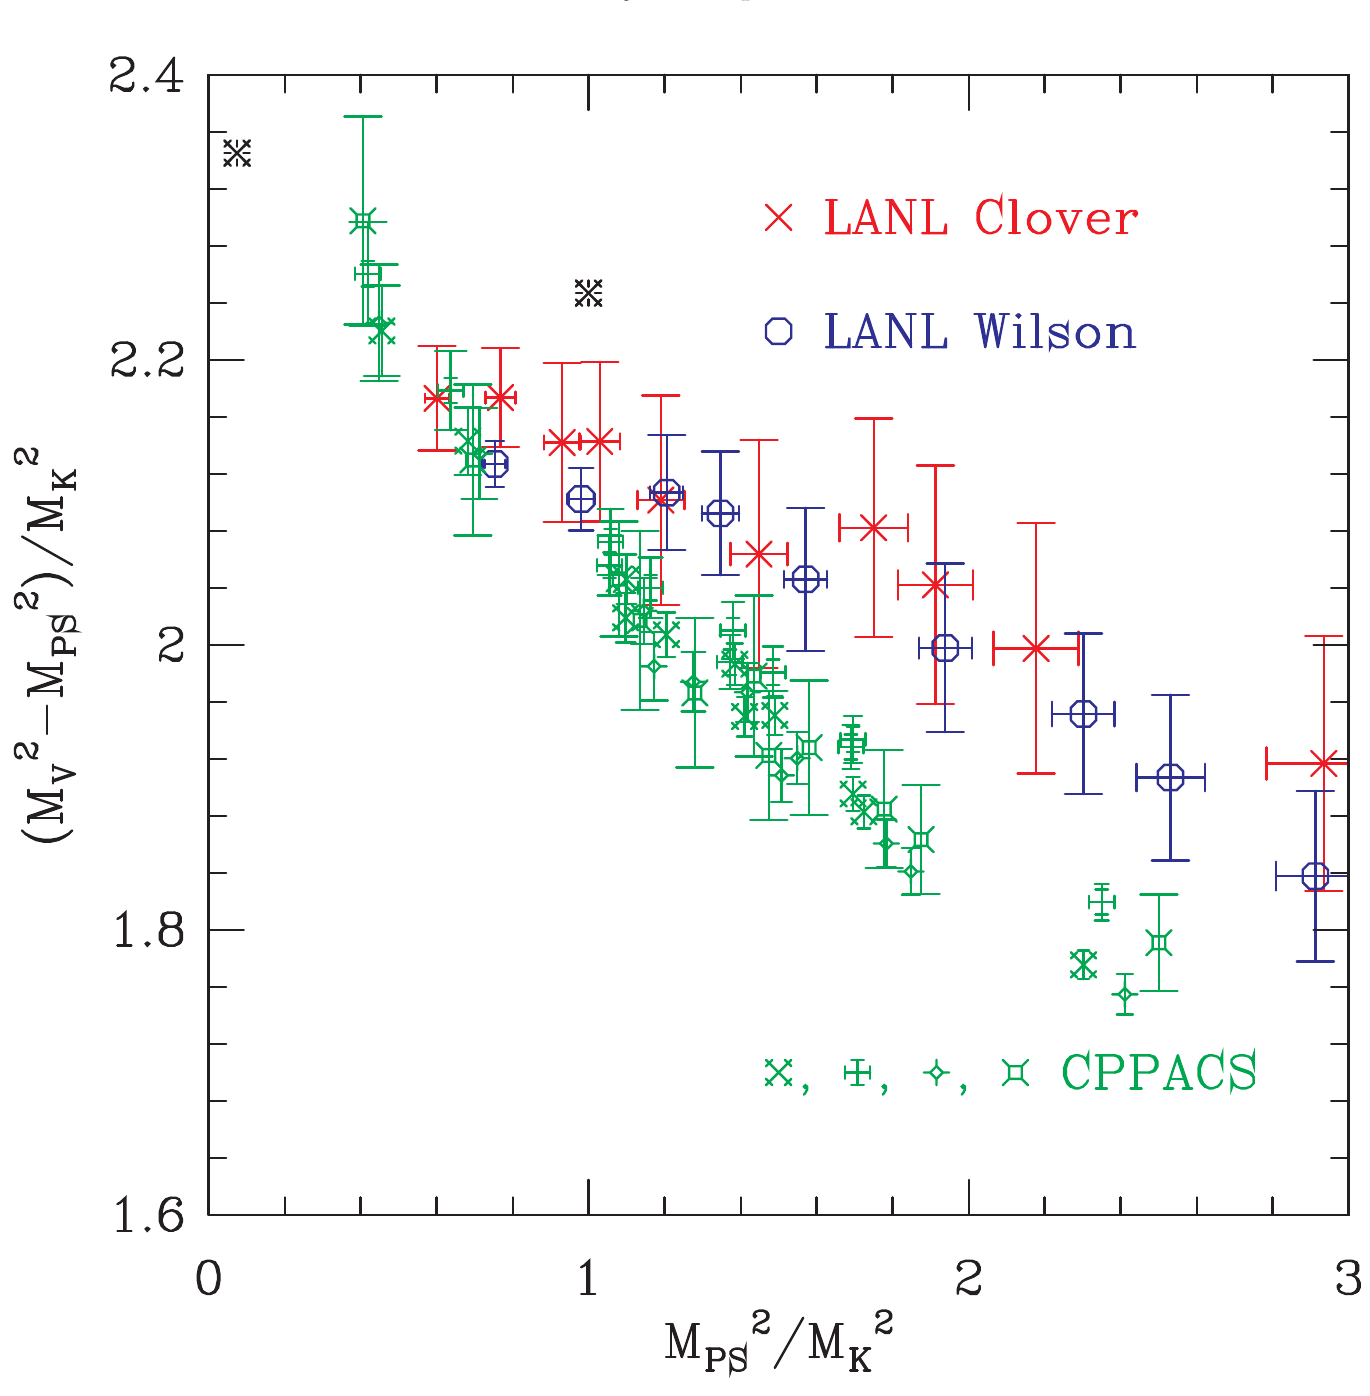
\includegraphics[width=0.8\textwidth]{images/fig26.png}
\caption{Hyperfine splittings in the meson sector. Quenched data from (i) LANL collaboration with Wilson fermions (blue octagons) [156], (ii) LANL collaboration with tadpole improved clover fermions (red crosses) [162], and (iii) CP-PACS collaboration Wilson runs at $\beta = 5.9, 6.1, 6.25, 6.47$ (green fancy crosses, pluses, diamonds, and squares) [161]. The experimental points are shown by the symbol burst.}
\label{fig:26}
\end{figure}

On the other hand, the slope at any given point is independent of the lattice scale, and is therefore the more robust lattice prediction. For this reason the quantity $J \equiv M_V \, \partial M_V / \partial M_{PS}^2$ is commonly used as a test of the hyperfine splittings. Lattice data (for a review see [161]) gives values for $J$ that are $\sim 20\%$ too small. Another manifestation of this discrepancy will appear in Section~20 where I show that the estimates of $m_s$ fixed using $M_K$ versus $M_{K^*}$ (or $M_\phi$) differ by $\sim 15\%$.

The data shown in Fig.~\ref{fig:26} allow two comparisons. First, the octagons (blue points) and crosses (red) are LANL data from the same 170 quenched $32^3 \times 64$ lattices at $\beta = 6.0$ with the Wilson and tadpole improved clover Dirac actions [156,162]. One does not find any significant improvement with clover fermions. Second, the fancy crosses, pluses, diamonds, and squares (green points) are Wilson fermion data from CP-PACS collaboration at $\beta = 5.9, 6.1, 6.25, 6.47$ [161]. The data at the four $\beta$ values are consistent. Both comparisons imply that the smaller splittings are not due to discretization errors.

The data in Fig.~\ref{fig:26} also show a difference between the CP-PACS and LANL Wilson fermion results at quark masses heavier than $m_s$. This is surprising since in this regime both collaborations have reliable measurements of the vector and pseudoscalar masses. The culprit is the lattice scale. It turns out that the estimate of $1/a$ from LANL data is 3\% larger compared to the value obtained by an interpolation of the CP-PACS data. Adjusting the LANL scale shifts their data as a whole and makes all the results overlap.

The conclusion, from this and other quenched data, is that the splittings come out too small. Even though the size of discretization errors is, in my opinion, not fully resolved, the deviations are thought to be mostly due to the use of the quenched approximation.

The most extensive discussion of the mass-splittings in the baryon octet and decuplet using the Wilson action is given in [156]. Note that since this calculation was done at only one $1/a \approx 2.3$ GeV, therefore discretization errors are not resolved. There are two important observations. (i) The mass splittings in the baryon octet show significant non-linearities, for example the dependence of $M_\Sigma - M_\Lambda$ on the quark mass is shown in Fig.~\ref{fig:27}.

\begin{figure}[htbp]
\centering
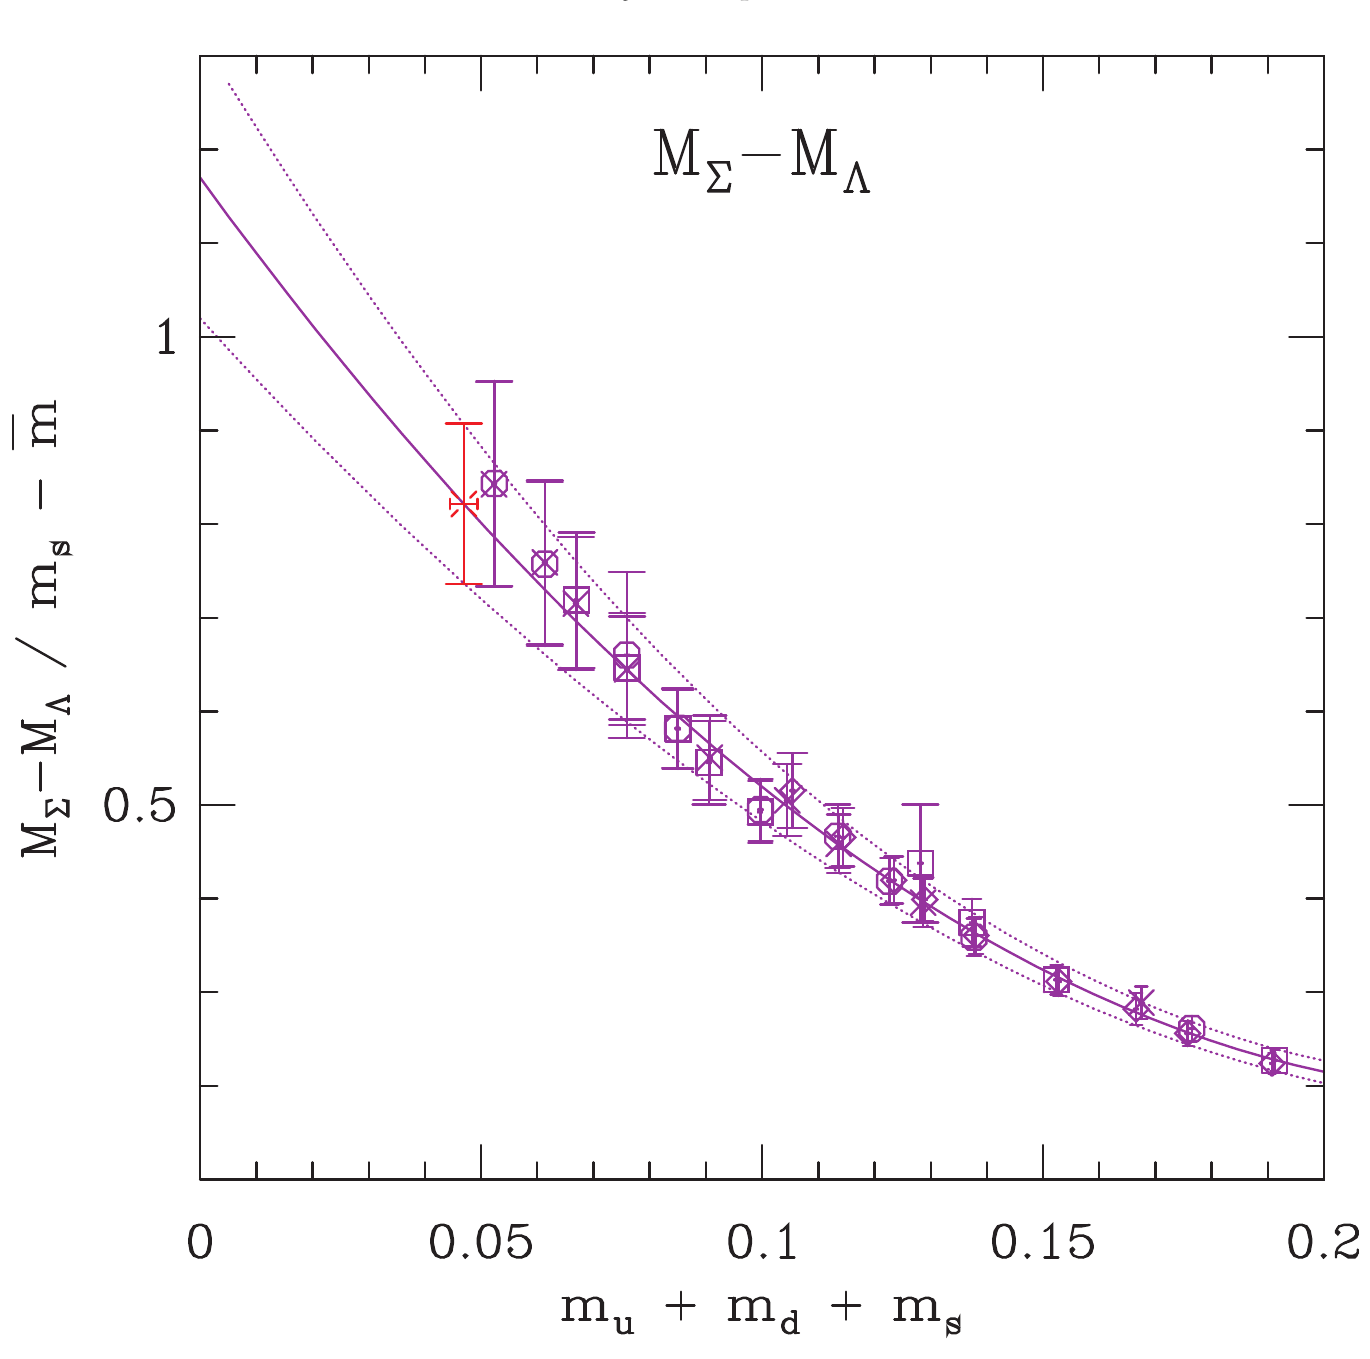
\includegraphics[width=0.8\textwidth]{images/fig27.png}
\caption{Quadratic fit to $(M_\Sigma - M_\Lambda)/(m - m_s)$, including baryons composed of completely non-degenerate quarks [156]. The value extrapolated to the physical point is shown by the burst symbol at the extreme left. The linear relations shown in Eq.~\eqref{eq:chiral} would predict a constant value.}
\label{fig:27}
\end{figure}

The non-linear terms significantly increase the splittings, and extrapolations to $m$ give results roughly consistent with experimental values. (ii) The decuplet baryon masses show a behavior linear in $m_1 + m_2 + m_3$, and the splittings come out too small for either choice $m_s(M_K)$ or $m_s(M_\phi)$.

The state-of-the-art Wilson fermion data have been obtained by the CP-PACS collaboration. Data have been obtained at four values of the lattice spacing so a reliable extrapolation to $a = 0$ can be made. Unfortunately, the data, in particular the baryon mass-splittings have not yet been fully analyzed so some of the observations presented here should be considered preliminary. Fig.~\ref{fig:28}, taken from Yoshie's review at LATTICE 97 [161], is CP-PACS's version of the chiral fits.

\begin{figure}[htbp]
\centering
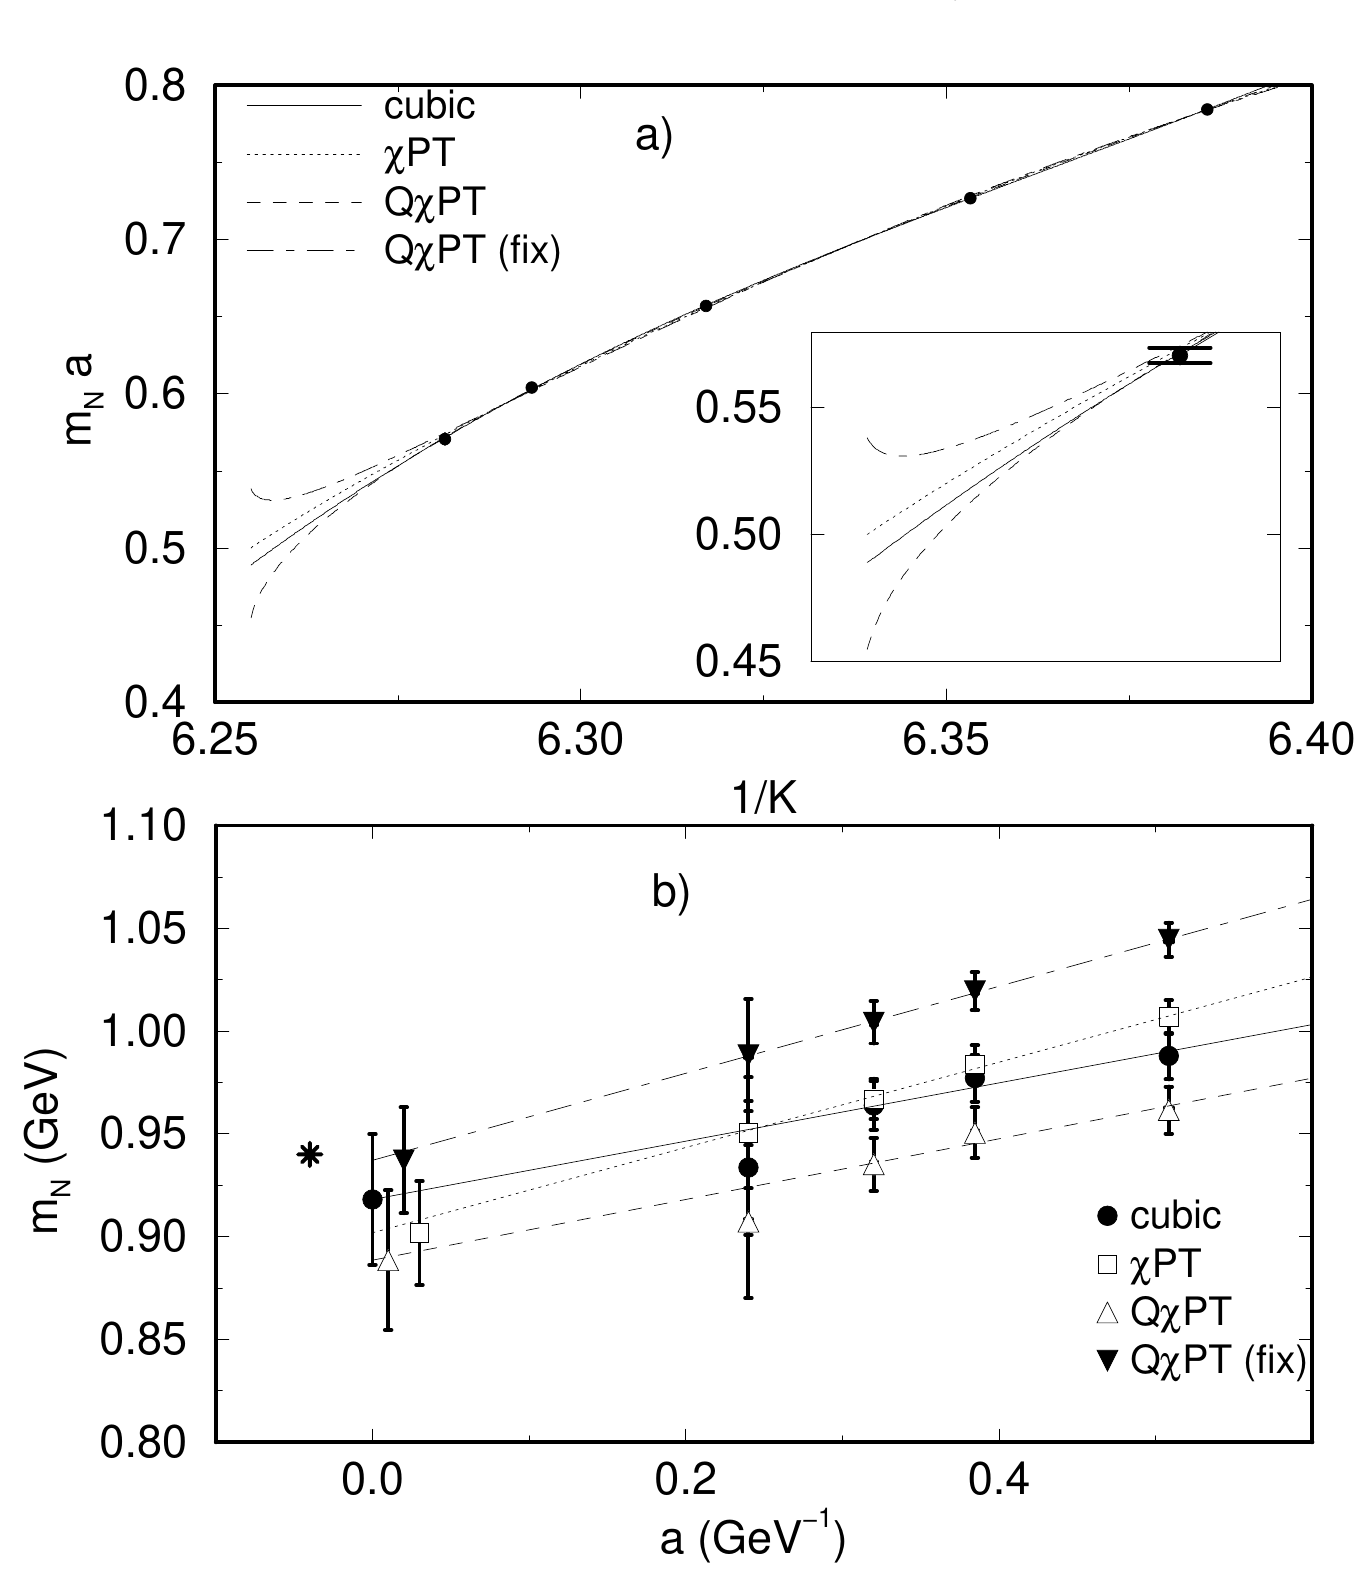
\includegraphics[width=0.8\textwidth]{images/fig28.png}
\caption{(A) Chiral fit to $M_{nucleon}$ data by the CP-PACS collaboration using the Wilson gauge and fermion actions. The data show negative curvature, though more points are needed to resolve between the cubic fit $M_N = c_0 + c_1 M_\pi + c_2 M_\pi^2 + c_3 M_\pi^3$, and $\chi$PT ($c_1 = 0$), Q$\chi$PT ($c_3 = 0$), $\chi$PT (fix) ($c_1 = -0.53$) fits. (B) Continuum extrapolation of the nucleon mass obtained using the different chiral expressions are shown in (A). The figures are reproduced from [161].}
\label{fig:28}
\end{figure}

They find that in the range $m_s/4 - m_s$ only the nucleon and the $\Lambda$ particles show any significant curvature. Even though data at more values of the quark mass are required to resolve the form of the leading higher order correction, the conclusion of their analyses is that the negative curvature found in their fits to nucleon data is sufficiently large to change the quenched estimate of $M_N / M_\rho$ to almost perfect agreement with the experimental value $\sim 1.22$. (This negative curvature was not seen/resolved in calculations reported before 1997, consequently a higher value in the range $1.3 - 1.4$ was usually reported.) Their extrapolation to $a = 0$ of results with different chiral fits is shown in Fig.~\ref{fig:29}.

\begin{figure}[htbp]
\centering
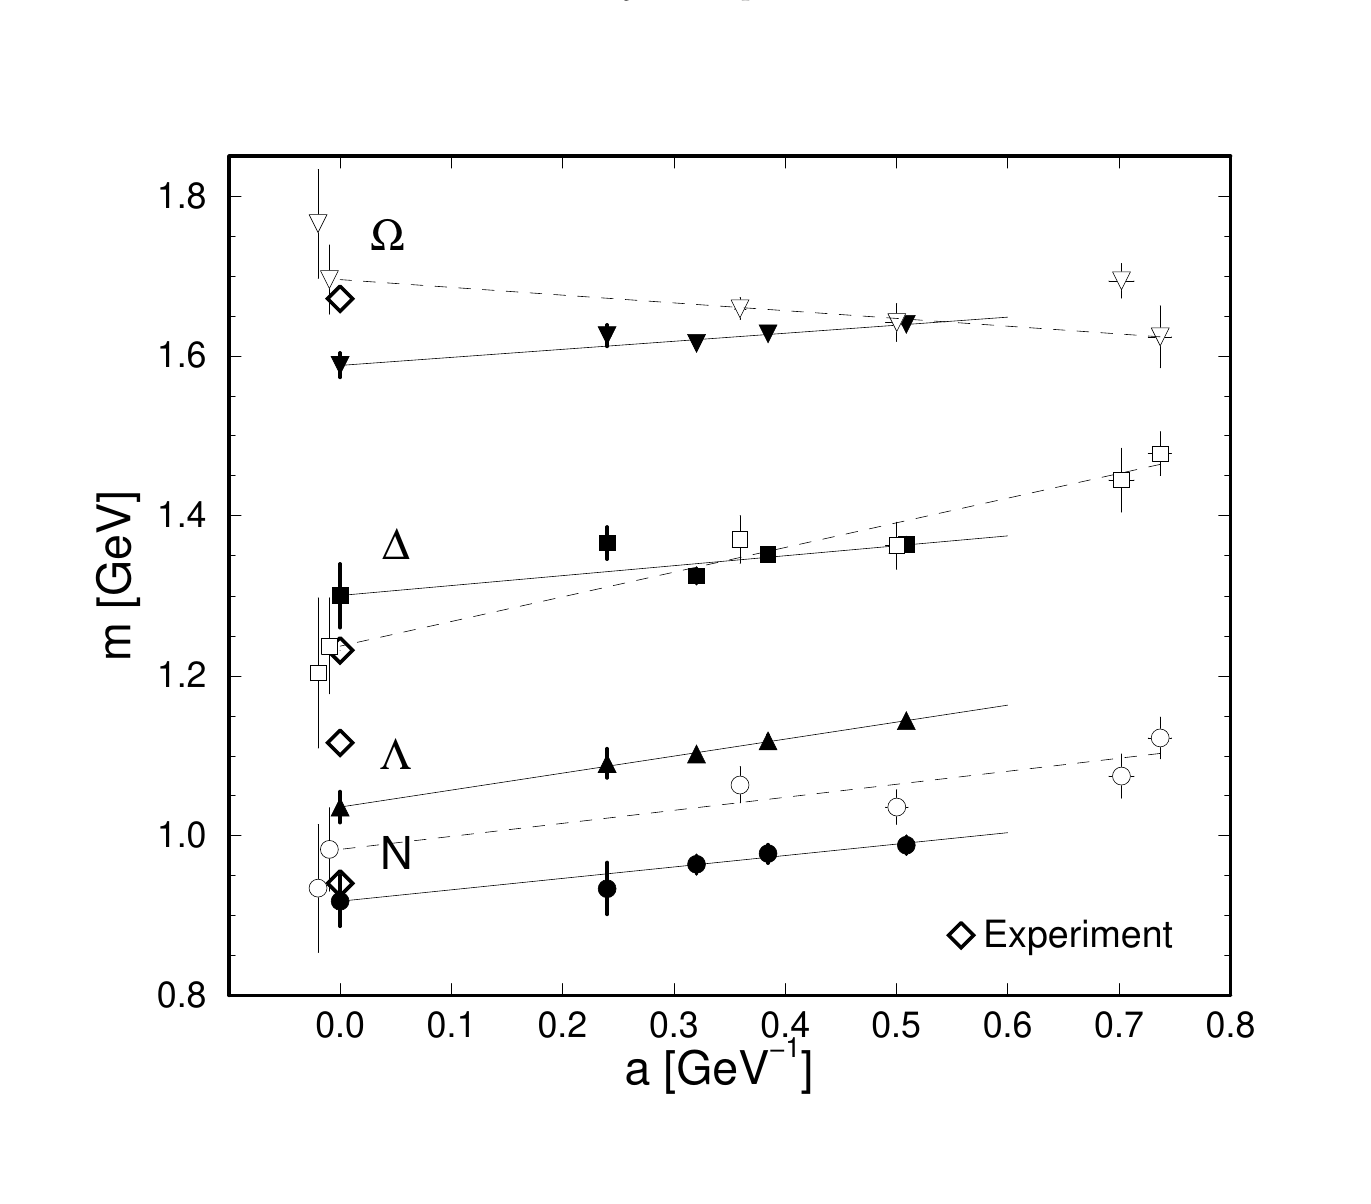
\includegraphics[width=0.8\textwidth]{images/fig29.png}
\caption{Continuum extrapolation of the nucleon, $\Lambda$, $\Delta$, and $\Omega$ masses obtained by the CP-PACS collaboration. The scale $a$ is set by $M_\rho$. The previous best results by the GF11 collaboration (unfilled symbols) are also shown. Experimental values are shown by the symbol diamond. Figure reproduced from [161].}
\label{fig:29}
\end{figure}

Second, they confirm that the decuplet masses are linear in the quark masses, and the splittings, even after extrapolation to $a = 0$, come out too small with either $m_s(M_K)$ or $m_s(M_\phi)$. Their full analyses on splittings in the baryon octet will appear soon.

A final summary of the quenched results taken from [161] using the Wilson action is given in Fig.~\ref{fig:30}.

\begin{figure}[htbp]
\centering
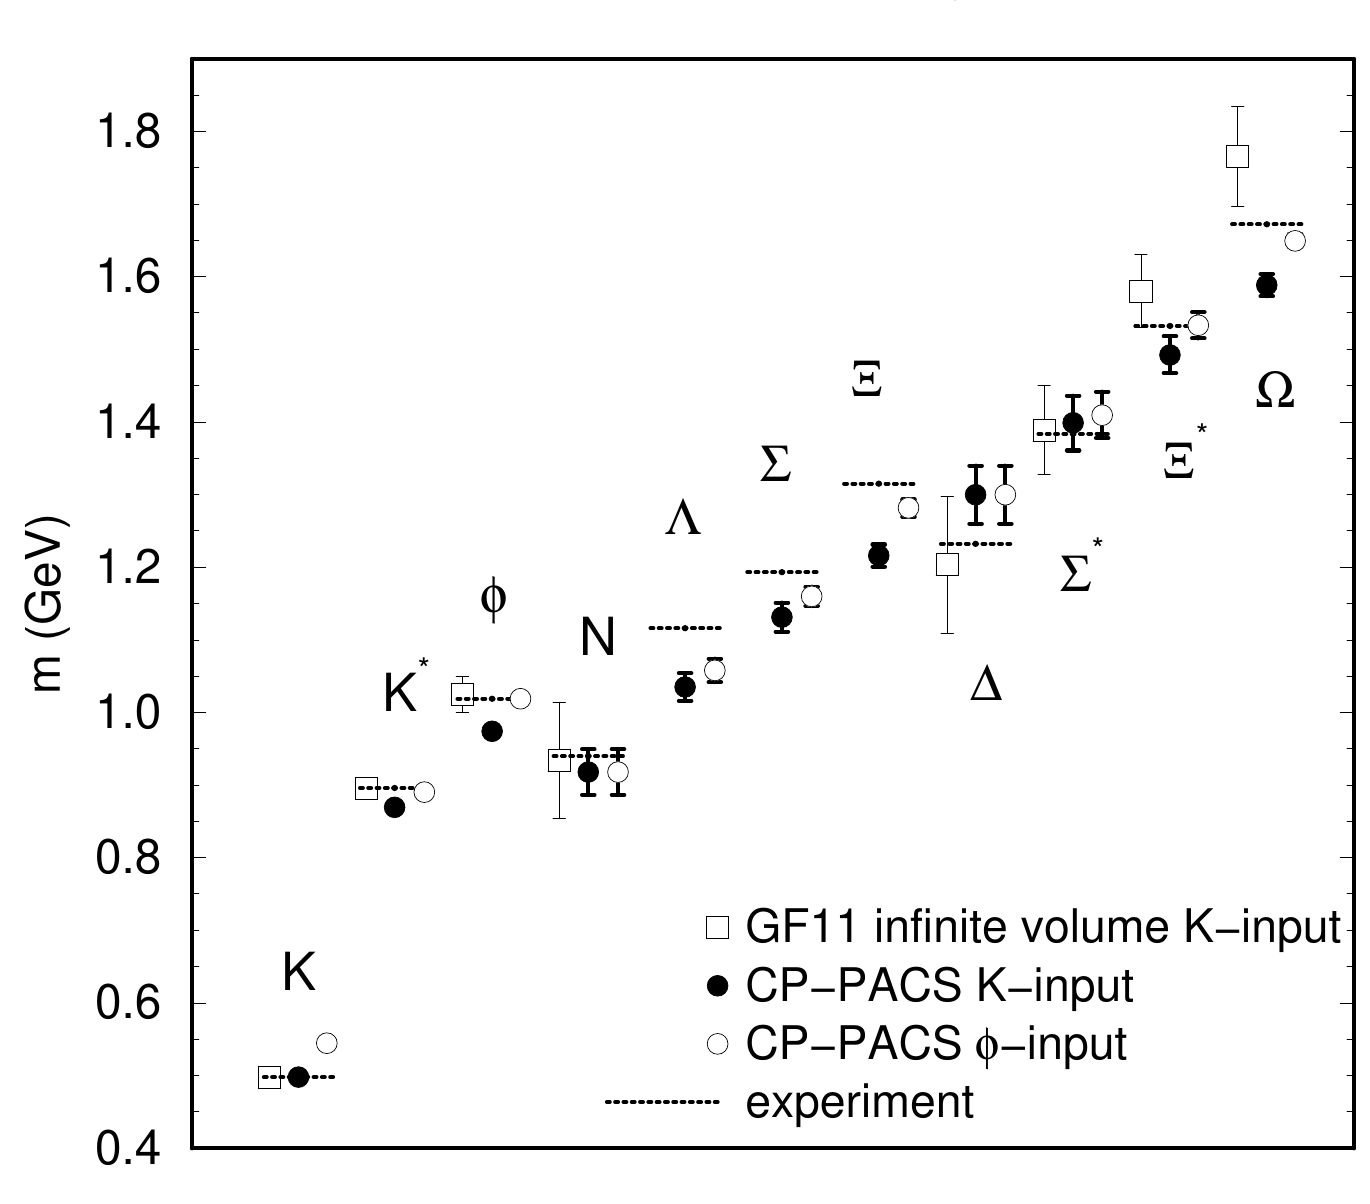
\includegraphics[width=0.8\textwidth]{images/fig30.png}
\caption{State-of-the-art results from the CP-PACS collaboration for the meson and baryon masses after $a = 0$ extrapolation and using Wilson fermions. The scale $a$ is set using $M_\rho$ and $m$ using $M_\pi$. Results are shown for two ways of setting $m_s$ --- $M_K$ and $M_\phi$ and it is clear that neither give correct splittings in the baryon octet and decuplet. The data are reproduced from [161].}
\label{fig:30}
\end{figure}

This figure compares the recent CP-PACS results extrapolated to $a = 0$ with the previous best calculation by the GF11 collaboration. The main lesson to be learned from this plot is that there does not seem to be a value of the strange quark mass that allows a matching of all the meson and baryon states. I shall come back to this point when discussing the extraction of quark masses. The obvious question is --- is this deviation an artifact of the quenched approximation? My view is that we still do not have full control over the quenched data, and therefore cannot point to quenching as the sole culprit. For example, the definition of $m_q$ itself has corrections of $O(m_q a)$, incorporating which would change the nature of the chiral fits. To fully understand the discretization errors we need to wait for similarly good quality data with the staggered and $O(a)$ improved clover formulations before claiming definitive quenched values.

As of this writing dynamical simulations have begun in earnest, but precise quantitative results at a number of values of $a$ and with different actions are lacking. Thus, I feel it is too early to draw any conclusions from them. For a status report on $n_f = 2$ results see the recent reviews by Yoshie and Gottlieb [161,160].

\section{Decay Constants}

In addition to the extraction of masses from the rate of exponential decay of the 2-point correlation function, the amplitudes $\langle n | O | 0 \rangle$ give decay constants. For example, the axial current matrix element $\langle \pi | A_\mu(x) | 0 \rangle = i f_\pi p_\mu \exp(i p \cdot x)$ gives the pion decay constant. Some of the recent results for decay constants have been reviewed by Prof.\ Martinelli at this school, and other recent reviews can be found in [163,164]. The technical points I would like to explain here are the reasons why the errors in decay constants are much larger than those in the determination of the masses. First, from Eq.~\eqref{eq:2pt} one notes that for a 1\% error in the determination of the mass, the fractional error in the decay amplitude is $\approx \exp(0.01 m \tau) - 1 \approx 0.005 m \tau$. Since fits typically have $m\tau \approx 5$ for $1/a \sim 2$ GeV lattices, the error in the decay constant is $\sim > 3\%$. Second, for any given configuration, the correlation function is highly correlated in $\tau$. Plotting $\log(\Gamma(\tau))$ for each individual configuration one notes that the dominant fluctuation is in the overall normalization, i.e., the amplitude. A very rapid growth in these fluctuations with decreasing $m_q$ is, in fact, the signal for exceptional configuration as discussed in Section~10. These two sources of error combine to produce a statistical error in decay constants that is much larger than in the extraction of $M_{eff}$. To this one has to add a systematic uncertainty coming from the renormalization constants for the local currents.

\section{Lattice Calculations of the Glueball Spectrum}

The existence of glueballs, hadronic states composed mainly of gluons, is a major untested prediction of QCD. Assuming QCD is the correct theory, we can determine the quantum numbers of a vast number of possible glueball states, but cannot yet calculate their masses, or their mixing with $q\bar{q}$, $qq\bar{q}\bar{q}$, \ldots{} states, or understand in detail the production and decay mechanisms. Various models like bag models, flux tube model, sum rules etc.\ give estimates of masses that differ significantly from each other and the reliability of these calculations is poor. A somewhat dated summary of the theoretical expectations, compiled by Burnett and Sharpe, can be found in [165]. The lack of knowledge of properties of glueballs does not help the experimentalists who have to isolate these states from the myriad of meson states in the $1-2.5$ GeV region. Clearly, LQCD calculations can play a vital role by calculating the spectrum and the mixing with $q\bar{q}$ mesons.

The first goal of LQCD has been to calculate the quenched spectrum in a world in which the mixing with quark states is turned off. I shall concentrate on just the $0^{++}$ and $2^{++}$ states as these have been studied most extensively. The glueball operators $O$ are constructed out of Wilson loops. Consider an $n \times m$ Wilson loop $W^{n,m}_{xy}$ lying in the $xy$ plane. Then the rotationally invariant sum $W^{n,m}_{xy} + W^{n,m}_{yz} + W^{n,m}_{zx}$ projects onto the $0^{++}$ state, while $W^{n,m}_{xy} - W^{n,m}_{yz}$ and its permutations project onto $2^{++}$. The signal in the 2-point correlator can be improved by taking a suitable linear combination of different sized loops that maximize the overlap with physical glueball states. One such strategy is discussed in [166]. Unfortunately, the statistical signal in glueball correlation functions is much weaker than that for meson and baryon correlation functions. Even with a sample of $O(10^5)$ independent configurations, the signal does not extend beyond $\tau \sim 10$ or $M\tau \sim 6$ and one barely has a ``plateau'' in the effective mass plot. The reason for this poor signal in glueball correlation functions is that they measure the fluctuations in the vacuum corresponding to the creation and propagation of a virtual glueball, whereas in meson and baryon correlators the quarks in the propagators are added as external sources.

The more recent, high statistics results for $M_{0^{++}}$ and $M_{2^{++}}$ states have been taken from Refs. [166--169]. The data and the extrapolation to $a = 0$ are shown in Fig.~\ref{fig:31}.

\begin{figure}[htbp]
\centering
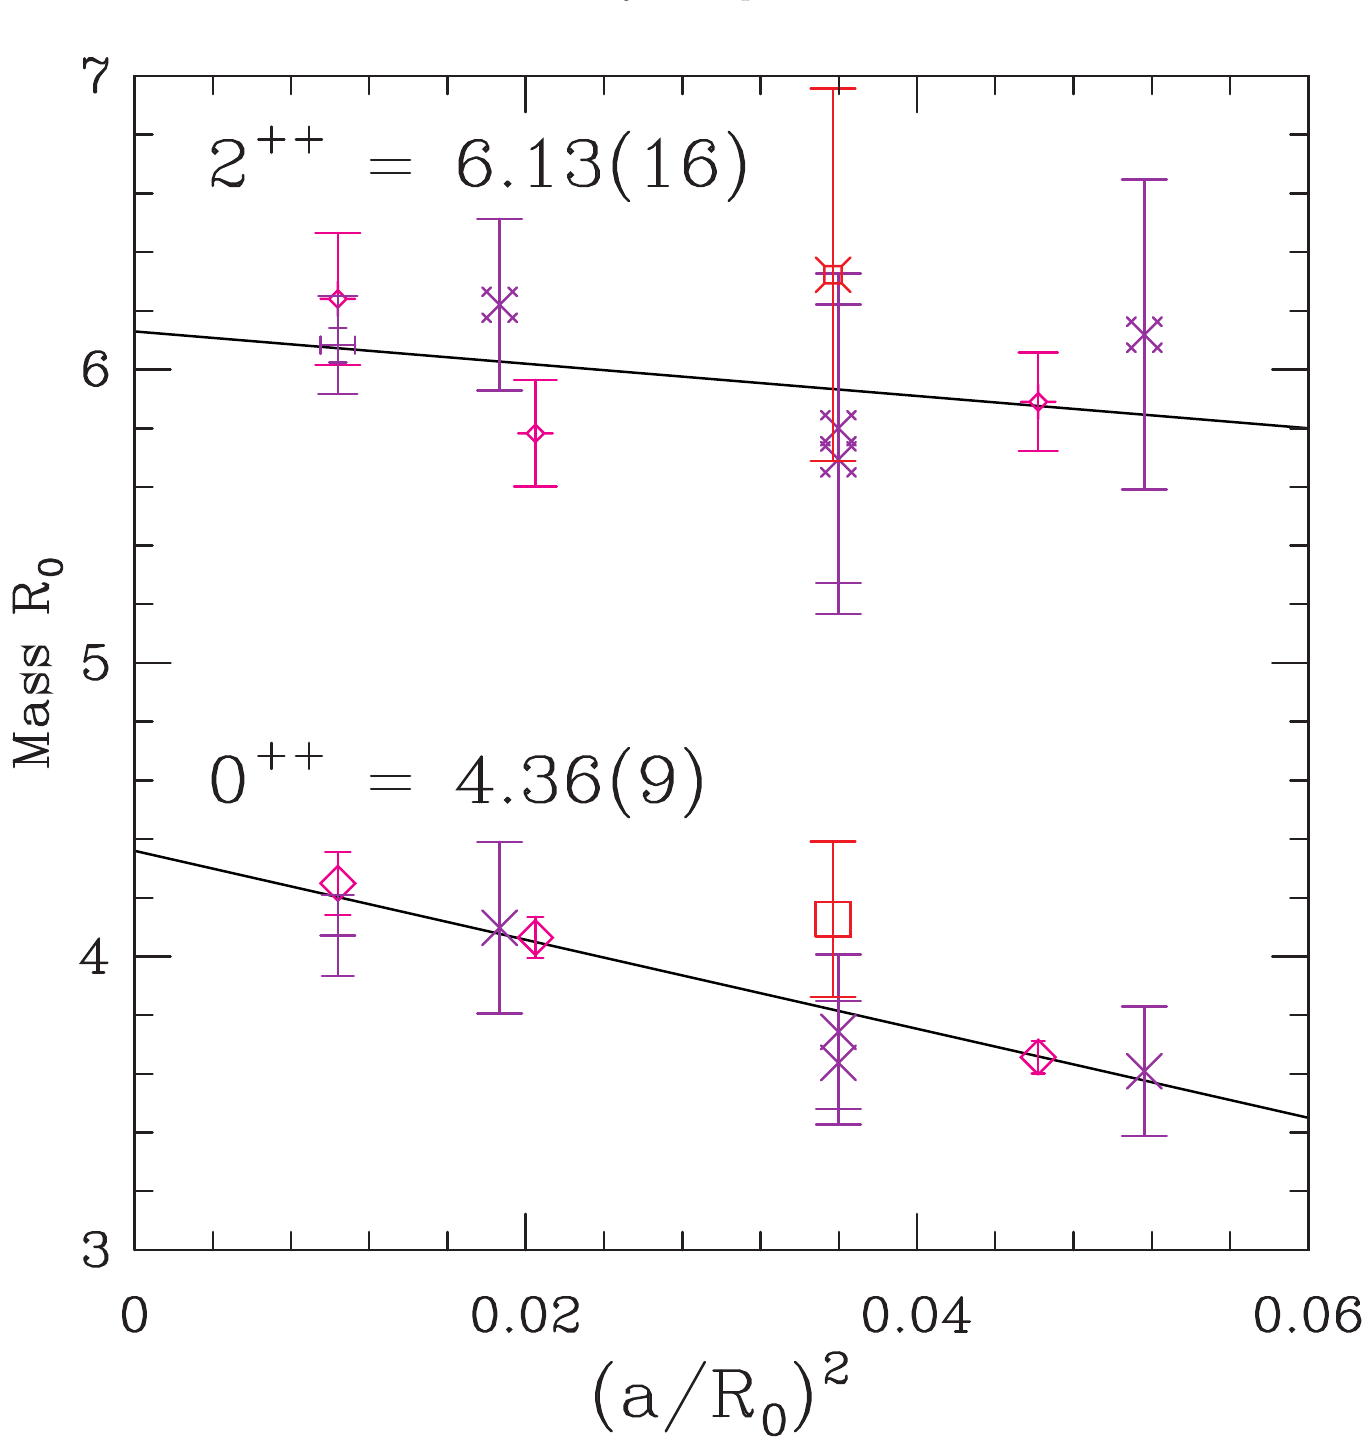
\includegraphics[width=0.8\textwidth]{images/fig31.png}
\caption{Extrapolation of $0^{++}$ and $2^{++}$ glueball mass data to $a = 0$. The data are from UKQCD-WUPPERTAL collaboration (crosses), GF11 collaboration (diamond), and Los Alamos collaboration (squares). The lattice scale is set using $R_0$ which is related to the string tension by $1/R_0 = \sqrt{\sigma}/1.18$.}
\label{fig:31}
\end{figure}

In this plot I have chosen to set the lattice scale using $R_0 = 1.18/\sqrt{\sigma}$, where $\sigma$ is the string tension [170]. The figure makes it clear that the lattice data from the various collaborations are completely consistent, though the statistical quality of the GF11 data [169] is much higher. A fit in $a^2$, the leading discretization error, gives $M_{0^{++}} R_0 = 4.36(9)$ and $M_{2^{++}} R_0 = 6.13(16)$ for the continuum limit of the quenched theory. To obtain masses in physical units one needs to choose a value for $R_0$ or equivalently $\sigma$. This brings us back to the overall scale uncertainty inherent in all quenched calculations. There are two questions relevant to this analysis (i) what value should one choose for $\sigma$, and (ii) by how much would the results change if one had used a different quantity like $M_\rho$ or $\Lambda_{QCD}$ to set the scale? The two most quoted results are the following. The UKQCD-WUPPERTAL collaboration use $1/R_0 = 373$ MeV based on choosing $\sqrt{\sigma} = 440$ MeV and get $M_{0^{++}} = 1626(34)$ and $M_{2^{++}} = 2286(60)$ MeV [170]. The updated GF11 collaboration estimates are $M_{0^{++}} = 1648(58)$ and $M_{2^{++}} = 2273(116)$ MeV using $\Lambda^{(0)}_{QCD} = 235(6)$ MeV which is based on $M_\rho$ to set the scale [171]. Thus, the estimates of the two groups are consistent and agree with the fit shown in Fig.~\ref{fig:31}. Therefore, in my view, based on these fits, the current combined lattice estimate is $M_{0^{++}} = 1640(30)(160)$ MeV and $M_{2^{++}} = 2280(60)(230)$ MeV, where I have added a second systematic error of 10\% to take into account the scale uncertainty inherent to quenched simulations.

\section{Improved action Results on Anisotropic lattices}

To alleviate the problem that the signal in glueball 2-point correlation functions falls rapidly, Peardon and Morningstar have carried out simulations on anisotropic hypercubic lattices, with $a_t \ll a_s$ [172]. The advantage of this trick is the following. Assume that there exists an approximate plateau in $M_{eff}(\tau)$ between $\tau = 2-4$ in an isotropic lattice simulation before the signal degrades to noise. Such a plateau is hard to infer from three time-slices. On the other hand for $a_s/a_t = 5$ lattices, one has roughly 11 time-slices to play with, thereby greatly increasing the confidence in the estimate. Using anisotropic lattices does introduce an additional parameter into the analyses, $a_s/a_t$ or the velocity of light. This they fix non-perturbatively using the measured potential in spatial and temporal directions.

\begin{figure}[htbp]
\centering
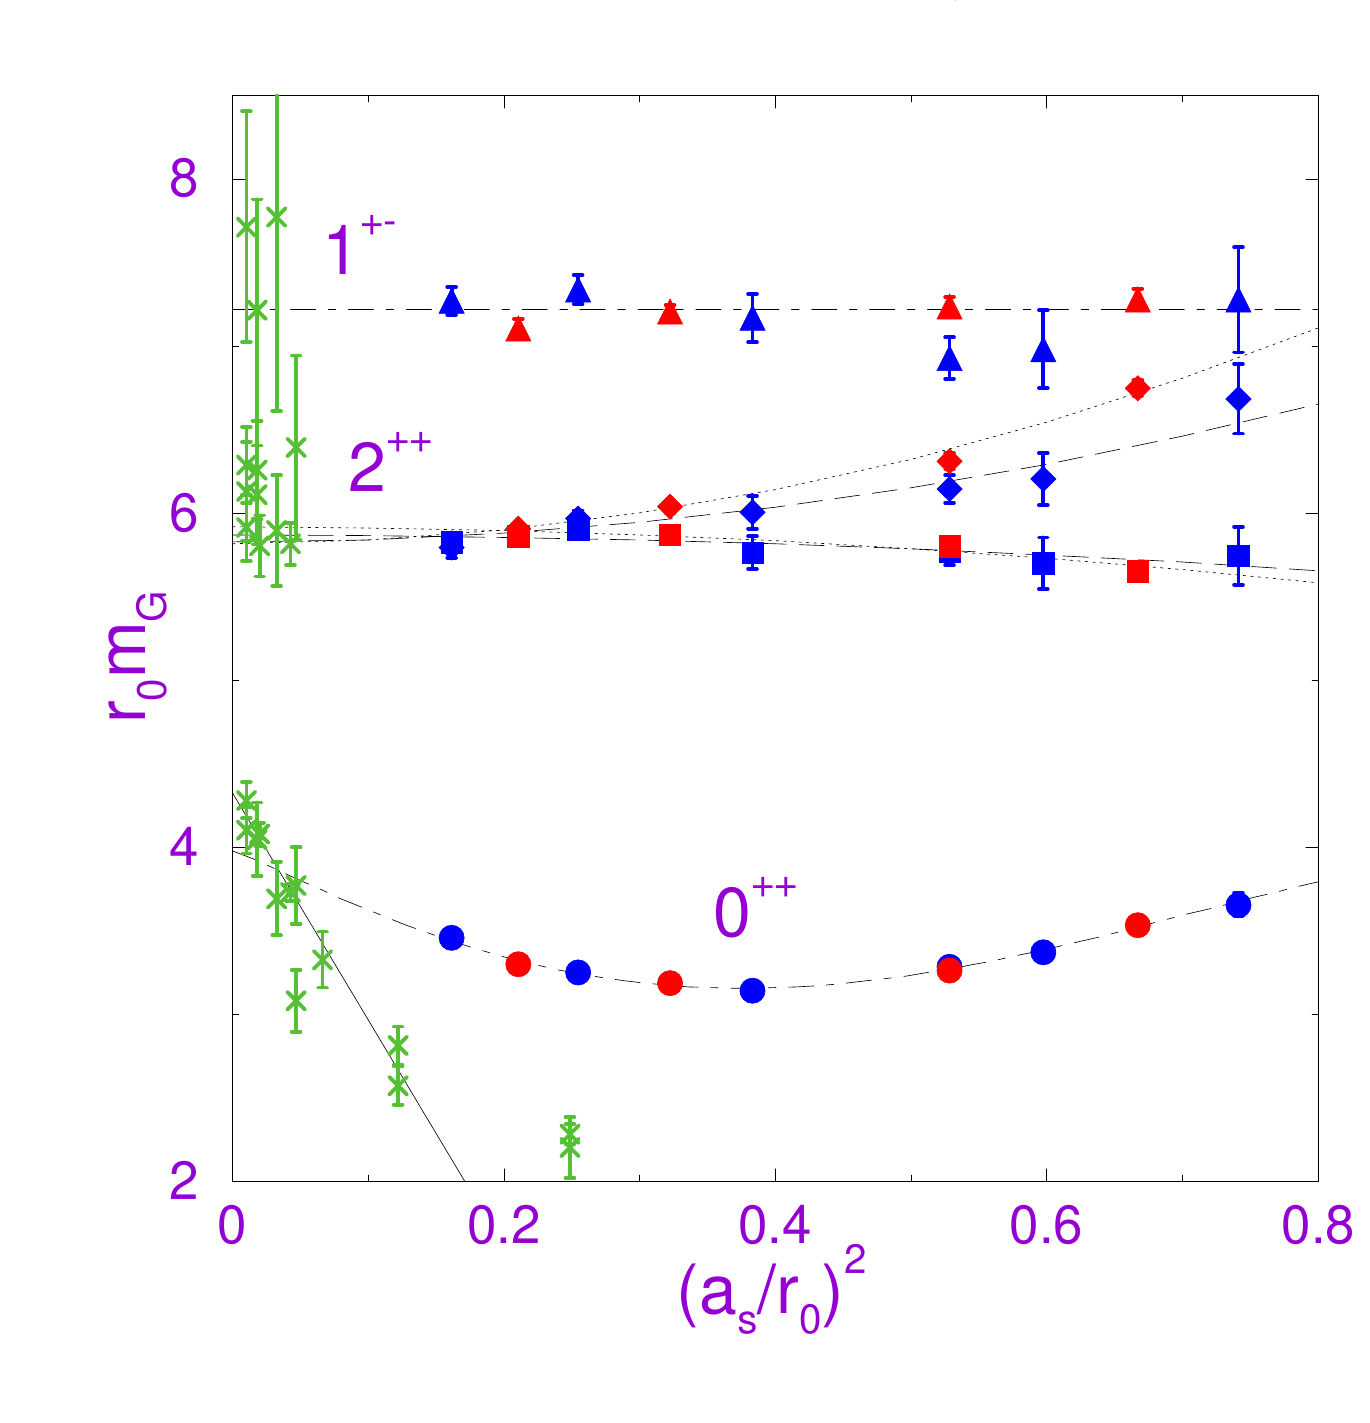
\includegraphics[width=0.8\textwidth]{images/fig32.png}
\caption{Glueball mass estimates in terms of $R_0$ against the lattice spacing $(a_s/R_0)^2$. Results from the $\xi = 5$ simulations for the lattice irreps $A_1^{++}$ ($0^{++}$), $E^{++}$, $T_2^{++}$ ($2^{++}$), and $T_1^{+-}$ ($1^{+-}$) are labeled $\circ$, $\square$, $\star$, and $\triangle$ (blue), respectively. The corresponding symbols in red indicate the results from the $\xi = 3$ simulations. Data from Wilson action simulations taken from Refs. [167--169] are shown using green crosses. The dashed, dotted, and dash-dotted curves indicate extrapolations to the continuum limit obtained by fitting to the $\xi = 3$ data, the $\xi = 5$ data, and all data, respectively. The solid line indicates the extrapolation of the Wilson action data to the continuum limit.}
\label{fig:32}
\end{figure}

The second improvement they make is to tune the action. They transcribe the tadpole improved L\"uscher-Weisz glue action, Eq.~12.14, on to anisotropic lattices and include the plaquette in both the fundamental and adjoint coupling space. The motivation for the latter is to avoid the phase transition in the fundamental-adjoint space as discussed in Section~15.

Their new data [139] confirms that including a negative adjoint coupling does improve the scaling in $M_{0^{++}}$.

Their results, prior to those including a negative adjoint coupling, are shown in Fig.~\ref{fig:32}. The advantage of improved action and anisotropic lattices is clearly visible. First, the calculations can be performed on much coarser lattices. Second, the discretization errors are much smaller. Lastly, the values after extrapolation to $a = 0$ are consistent with conventional methods. Their estimates $M_{0^{++}} R_0 = 3.98(15)$ and $M_{2^{++}} R_0 = 5.85(2)$, when combined with their estimate $R_0 = 410(20)$ MeV, are consistent with the values from conventional simulations given in the previous section. Thus, their results provide another confirmation of the quenched estimates.

Let me end this discussion of gluey states with pointers to other interesting calculations. Results for other spin-parity glueball states can be found in [168,172,173]; and for hybrid states in [173--176].

\section{Mixing between scalar quarkonia and glueballs}

The phenomenologically important question is whether the lattice estimates can help pin down which of the two experimental candidates, $f_0(1500)$ or $f_0(1710)$, is the scalar glueball. The answer, using just the above quenched estimates, is no. The reason, in addition to the fact that the above estimates overlap with both candidates, is that effects of mixing with scalar quarkonia have not been included. Lee and Weingarten have initiated a study of mixing by calculating the two-point functions $\langle S(\tau) S(0) \rangle$ and $\langle G(\tau) S(0) \rangle$ where $S$ is the scalar density $(u\bar{u} + d\bar{d})/\sqrt{2}$ or $s\bar{s}$ and $G$ is the $0^{++}$ glueball operator [171]. The statistical quality of these very hard calculations is not yet good. Lee and Weingarten, therefore, diagonalize an approximate $3 \times 3$ matrix that is obtained mainly from a phenomenological analysis. They then find that mixing raises $M_{0^{++}}$ by $\sim 64$ MeV, i.e.\ $M_{0^{++}}$ changes from 1640 to 1704 MeV. Also, the associated wavefunctions of the mixed states explain some of the unexpected features of decays, like why the $KK$ decay mode of $f_0(1500)$ is suppressed and why $\Gamma(J/\psi \to \gamma f_0(1710)) > \Gamma(J/\psi \to \gamma f_0(1390)) \gg \Gamma(J/\psi \to \gamma f_0(1500))$. Consequently, Lee and Weingarten predict that $f_0(1710)$ is dominantly ($\sim 75\%$) a glueball.

In obtaining these predictions, they neglected mixing with other (multiparticle) states and decay widths in the mixing matrix and quenching errors in the lattice calculations. These, Lee and Weingarten claim on the basis of phenomenological arguments, are small and do not change their central conclusion. Hopefully, future LQCD calculations will provide a much better quantitative validation of their prediction.

\section{Mass Inequalities}

In addition to getting hard numbers, LQCD (actually Euclidean field theory) has also prompted the derivation of rigorous mass-inequalities. The first such was derived by Weingarten showing that the pion is the lightest meson state of non-zero isospin in QCD [177]. Consider the 2-point correlation function for mesons, i.e.\ $O = \bar{u}\Gamma d$ where $\Gamma$ can be any one of the 16 elements of the Clifford algebra. Then
\begin{equation}
\begin{aligned}
\Gamma_{\Gamma}(\tau) &= \int d^3y\, \langle 0 | \bar{d}\Gamma u(\tau, y)\, \bar{u}\Gamma d(0, x) | 0 \rangle \\
&= \Tr\, S_F^d(0,x;\tau,y)\,\Gamma S_F^u(\tau,y;0,x)\,\Gamma \\
&= \Tr\, \Gamma\gamma_5 S_F^{d\dagger}(\tau,y;0,x)\,\gamma_5 \Gamma S_F^u(\tau,y;0,x).
\end{aligned}
\label{eq:18.4}
\end{equation}

For the special case of the pion, $\Gamma\gamma_5 = 1$, consequently $\Gamma_\pi(\tau)$ has the maximum value on each configuration. Furthermore, for $m_u = m_d$ it is the absolute square of the propagator. The other spin-parity states involve $\gamma$ matrices. Since these have both plus and minus signs, the various spinor terms in the trace have cancellations. The second property needed to translate this property of correlation functions into an inequality on masses is that the integration measure for QCD is positive, i.e.\ each configuration contributes with the same sign. Thus, $\Gamma_\pi(\tau) \ge \Gamma_\Gamma(\tau)$ for all $\tau$. Since, $\Gamma(\tau) \sim e^{-m\tau}$, the inequality implies that the pion is the lightest meson.

Concurrently, Witten and Nussinov derived further inequalities. Examples of these are
\begin{itemize}
  \item The electromagnetic mass shift in the pion is positive [179]. Specifically what is shown is that $V_\mu^3(k)V_\mu^3(-k) - A_\mu^3(k)A_\mu^3(-k) \ge 0$ for any Euclidean $k$.
  \item For mesons with valence flavors $A$ and $B$ the inequality $2M_{AB} \ge M_{AA} + M_{BB}$ holds in the limit that annihilation into gluonic states can be neglected in the flavor singlet correlators [179,178].
\end{itemize}

Recently West has applied/extended these methods to glueballs [181]. He shows that $0^{++}$ is the lightest glueball state.
